%-----------------------------------------------------------------------------%
\chapter{\babTiga}
%-----------------------------------------------------------------------------%
Pada bab ini akan dijelaskan sekilas tentang \latex, beberapa perintah dasar \latex beserta cara menggunakan dan contoh-contohnya.

%-----------------------------------------------------------------------------%
\section{\latex~\textit{in Brief}}
%-----------------------------------------------------------------------------%
%Merujuk ke Tobias Oetiker \cite{tobi_latex}, Tex adalah sebuah program komputer yang dibuat oleh Donald E. Knuth.

Di Internet dapat dicari berbagai artikel yang menjelaskan apa dan sejarah \latex. Namun yang perlu dipahami adalah alasan menggunakan \latex~dalam penyusunan tugas akhir. Penggunaan \latex~diharapkan memudahkan penulis dalam membuat tugas akhir. Penulis diharapkan lebih fokus ke isi atau konten dari buku yang disusun. Dengan \latex!~penulis tidak perlu ribet dalam melakukan \textit{formatting} tulisan, pemberian halaman dan daftar isi, pembuatan daftar gambar dan tabel, serta pembuatan \textit{link} sitasi dan daftar referensi.

%-----------------------------------------------------------------------------%
\section{Perintah-Perintah Dasar \latex}
%-----------------------------------------------------------------------------%
Bagian ini berisi beberapa perintah dasar \latex~ beserta cara menggunakan dan contoh-contohnya.

\subsection{\textit{Formatting} Tulisan}
\begin{itemize}
\item Tulisan Tebal (\textit{Bold})\\
\textbackslash textbf\{\textit{argument}\} untuk menebalkan tulisan.\\
contoh:
\textbackslash textbf\{tulisan tebal\} $\rightarrow$ \textbf{tulisan tebal}

\item Tulisan Miring (\textit{Italic})\\
\textbackslash textit\{\textit{argument}\} untuk memiringkan tulisan.\\
contoh:
\textbackslash textit\{tulisan miring\} $\rightarrow$ \textit{tulisan miring}

\item Tulisan Bergaris Bawah (\textit{Underlined})\\
\textbackslash uline\{\textit{argument}\} untuk menggarisbahwahi tulisan.\\
contoh:
\textbackslash uline\{tulisan bergaris bawah\} $\rightarrow$ \uline{tulisan bergaris bawah}

\item Tulisan Menggantung ke Atas (\textit{Superscript})\\
\textbackslash textsuperscript\{\textit{argument}\} untuk membuat tulisan menggantung.\\
contoh:
\textbackslash textsuperscript\{tulisan menggantung\} $\rightarrow$ \textsuperscript{tulisan menggantung ke atas}

\item Tulisan Menggantung ke Bawah (\textit{Subscript})\\
\textbackslash textsubscript\{\textit{argument}\} untuk membuat tulisan menggantung.\\
contoh:
\textbackslash textsubscript\{tulisan menggantung\} $\rightarrow$ \textsubscript{tulisan menggantung ke bawah}

\item Tulisan yang Dicoret (\textit{Strike-through})
\textbackslash sout\{\textit{argument}\} untuk membuat tulisan tercoret.\\
contoh:
\textbackslash sout\{tulisan tercoret\} $\rightarrow$ \sout{tulisan tercoret}
\end{itemize}

\subsection{Memasukkan Gambar}
Untuk memasukkan gambar ke dalam dokumen, digunakan \textit{syntax} \textbackslash begin\{figure\} ... \textbackslash end\{figure\}. Berikut contoh memasukkan \textit{file} gambar \textit{bipartite.png} yang berada di dalam folder \textit{pics/diagram/}. Dari kode tersebut didapatkan hasil gambar \ref{fig:bipartite}. Label dapat diberikan di dalam \textit{figure}, sehingga untuk merujuk sebuah gambar dapat digunakan \textit{ref}. Contoh penggunaan \textit{ref}, misalkan \textbackslash ref\{fig:bipartite\} $\rightarrow$ \ref{fig:bipartite}.

\begin{lstlisting}
\begin{figure}
	\centering
	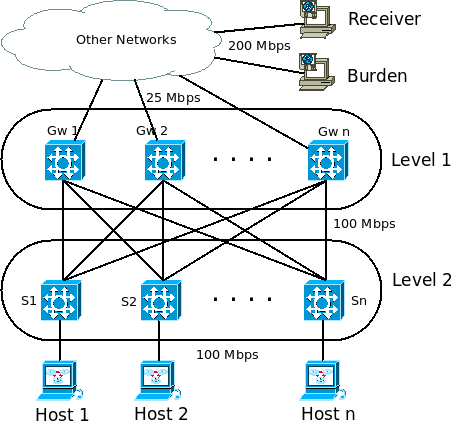
\includegraphics[width=0.6\textwidth]
		{pics/diagram/bipartite.png}
		\caption{Topologi \textit{Bipartite} untuk Pengukuran Fail-Over Delay}
	\label{fig:bipartite}
\end{figure}
\end{lstlisting}

\begin{figure}
	\centering
	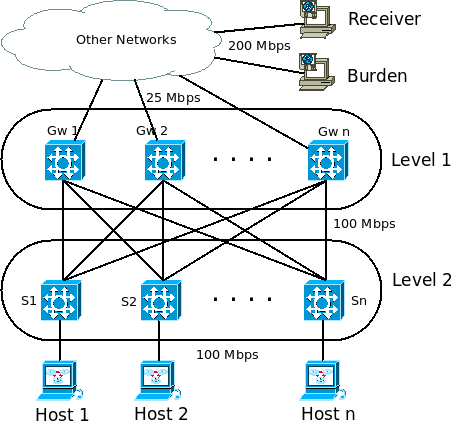
\includegraphics[width=0.6\textwidth]
		{pics/diagram/bipartite.png}
		\caption{Topologi \textit{Bipartite} untuk Pengukuran Fail-Over Delay}
	\label{fig:bipartite}
\end{figure}

\subsection{Membuat Tabel}
Untuk memasukkan tabel ke dalam dokumen, digunakan \textit{syntax} \textbackslash begin\{table\} ... \textbackslash end\{table\}

\begin{lstlisting}
\begin{table}
	\centering
	\caption{Jumlah \textit{Switch} dan \textit{Host} serta Jenis \textit{Traffic} untuk Setiap Pengukuran}
	\label{tab:tab1}
	\begin{tabular}{| l | r | r | r | c |}
		\hline
		Pengukuran & L1 & L2 & \textit{Host} & \textit{Traffic}\\ 
		\hline
		\textit{Fail-Over Delay} & 2 - 4  & 1 - 8 & 1 - 8 & ICMP Ping Tunggal\\
		\textit{Load Balance: Load Distribution} & 1 - 4 & 1 & 1 & 200 UDP \textit{Flows}\\
		\textit{Load Balance: Performance} & 1 - 4  & 1 - 8 & 1 - 8 & Data, Video, VoIP \textit{Flows}\\
		\textit{Overhead Size} & 2 & 1 & 1 & 25 - 150 UDP \textit{Flows}\\
		\textit{Memory Consumption: Switch} & 1 - 4  & 1 - 8 & 0 & -\\
		\textit{Memory Consumption: Host}  & 1 & 1 & 0 - 200 & - \\
		\hline
	\end{tabular}
\end{table}
\end{lstlisting}

\begin{table}
	\centering
	\caption{Jumlah \textit{Switch} dan \textit{Host} serta Jenis \textit{Traffic} untuk Setiap Pengukuran}
	\label{tab:tab1}
	\begin{tabular}{| l | r | r | r | c |}
		\hline
		Pengukuran & L1 & L2 & \textit{Host} & \textit{Traffic}\\ 
		\hline
		\textit{Fail-Over Delay} & 2 - 4  & 1 - 8 & 1 - 8 & ICMP Ping Tunggal\\
		\textit{Load Balance: Load Distribution} & 1 - 4 & 1 & 1 & 200 UDP \textit{Flows}\\
		\textit{Load Balance: Performance} & 1 - 4  & 1 - 8 & 1 - 8 & Data, Video, VoIP \textit{Flows}\\
		\textit{Overhead Size} & 2 & 1 & 1 & 25 - 150 UDP \textit{Flows}\\
		\textit{Memory Consumption: Switch} & 1 - 4  & 1 - 8 & 0 & -\\
		\textit{Memory Consumption: Host}  & 1 & 1 & 0 - 200 & - \\
		\hline
	\end{tabular}
\end{table}

\subsection{Notasi Matematika}
Untuk menuliskan notasi matematika, pada \latex digunakan \textit{syntax} \$ ... \$ untuk penggunaan di dalam paragraf dan \textbackslash begin\{equation\} ... \textbackslash end\{equation\} untuk penggunaan terpisah di luar paragraf. Sebagai contoh sebagai berikut.
\begin{itemize}
\item contoh 1:
\begin{lstlisting}
\begin{equation}
	metric_{i,j} = \frac{10^2}{(capacity_{E_{i,j}} - 	load_{E_{i,j}})}
	\label{eq:metric1}
\end{equation}
\end{lstlisting}
\begin{equation}
	metric_{i,j} = \frac{10^2}{(capacity_{E_{i,j}} - 	load_{E_{i,j}})}
	\label{eq:metric1}
\end{equation}
\item contoh 2:
\begin{lstlisting}
\begin{equation}
	f(x)=(x+a)(x+b)
	\label{eq:fx1}
\end{equation}
\end{lstlisting}
\begin{equation}
	f(x)=(x+a)(x+b)
	\label{eq:fx1}
\end{equation}
\item contoh 3
\begin{lstlisting}
\begin{subequations}
Maxwell's equations:
	\begin{align}
		B'&=-\nabla \times E,\\
		E'&=\nabla \times B - 4\pi j,
	\end{align}
	\label{eq:maxwell}
\end{subequations}
\end{lstlisting}
\begin{subequations}
Maxwell's equations:
	\begin{align}
		B'&=-\nabla \times E,\\
		E'&=\nabla \times B - 4\pi j,
	\end{align}
	\label{eq:maxwell}
\end{subequations}
\item contoh 4
\begin{lstlisting}[language=tex]
matriks $Adj$ digunakan untuk menggambarkan topologi jaringan  $G = (V,E)$, di mana $V = \{v_{1}, v_{2}, ..., v_{n}\}$ merupakan \textit{switch} dan $E = \{e_{1,1}, e_{1,2}, ..., e_{n,n}\}$ merupakan \textit{link} antar-\textit{switch}. Setiap $E_{i,j}$ menyimpan informasi \textit{metric} sesuai persamaan \ref{eq:metric1} . Hasil dari algoritma ini adalah jalur $T_{k,l}$ yang disimpan di dalam \textit{bucket Path} atau $T$. Setiap $T_{k,l}$ mempunyai nilai \textit{metric} sesuai persamaan \ref{eq:metric2}.
\end{lstlisting}
matriks $Adj$ digunakan untuk menggambarkan topologi jaringan  $G = (V,E)$, di mana $V = \{v_{1}, v_{2}, ..., v_{n}\}$ merupakan \textit{switch} dan $E = \{e_{1,1}, e_{1,2}, ..., e_{n,n}\}$ merupakan \textit{link} antar-\textit{switch}. Setiap $E_{i,j}$ menyimpan informasi \textit{metric} sesuai persamaan \ref{eq:metric1}. Hasil dari algoritma ini adalah jalur $T_{k,l}$ yang disimpan di dalam \textit{bucket Path} atau $T$. Setiap $T_{k,l}$ mempunyai nilai \textit{metric} sesuai persamaan 3.2.
\end{itemize} 

\subsection{Notasi Algoritma \textit{Pseudo-Code}}
Untuk menuliskan \textit{pseudo-code} digunakan \textit{syntax} \textbackslash begin\{algorithm\} ... \textbackslash end\{algorithm\}. Berikut contoh notasi \textit{pseudo code}.
\begin{lstlisting}
\begin{algorithm}
\caption{--- Find all possible path from graph G --- Adapted from DFS algorithm}\label{alg1}
\begin{algorithmic}[1]
\Require network topology $G = (V,E)$ represented in dictionary $Adj$, where $V, E$ represents DPID and link between DPID
\Ensure a routing table for source-destination DPID pairs represented in dictionary $T$
\State $T \leftarrow \{\}$
\Procedure{Per\textunderscore Source\textunderscore DFS}{$source, origin =$ None, $path \leftarrow []$}
  \If{$origin \equiv$ None}
    \State $origin \leftarrow source$
  \EndIf
  \For{$i \in M[source]$}
    \If{$i \in path \lor i \equiv origin$}
      \State continue
    \Else
      \If{$i \notin T[origin]$}
        \State $T[origin][i] \leftarrow [path + [i])]$
        \Else
          \State append $[path + [i])]$ to $T[origin][i]$
      \EndIf
      \State PER\textunderscore SOURCE\textunderscore DFS($i, origin, path + [i]$)
    \EndIf
  \EndFor
\EndProcedure
\For{$i \in Adj$}
  \State $path[i] \leftarrow \{\}$
  \State PER\textunderscore SOURCE\textunderscore DFS($i$)
\EndFor
\end{algorithmic}
\end{algorithm}
\end{lstlisting}

\begin{algorithm}
\caption{--- Find all possible path from graph G --- Adapted from DFS algorithm}\label{alg1}
\begin{algorithmic}[1]
\Require network topology $G = (V,E)$ represented in dictionary $Adj$, where $V, E$ represents DPID and link between DPID
\Ensure a routing table for source-destination DPID pairs represented in dictionary $T$
\State $T \leftarrow \{\}$
\Procedure{Per\textunderscore Source\textunderscore DFS}{$source, origin =$ None, $path \leftarrow []$}
  \If{$origin \equiv$ None}
    \State $origin \leftarrow source$
  \EndIf
  \For{$i \in M[source]$}
    \If{$i \in path \lor i \equiv origin$}
      \State continue
    \Else
      \If{$i \notin T[origin]$}
        \State $T[origin][i] \leftarrow [path + [i])]$
        \Else
          \State append $[path + [i])]$ to $T[origin][i]$
      \EndIf
      \State PER\textunderscore SOURCE\textunderscore DFS($i, origin, path + [i]$)
    \EndIf
  \EndFor
\EndProcedure
\For{$i \in Adj$}
  \State $path[i] \leftarrow \{\}$
  \State PER\textunderscore SOURCE\textunderscore DFS($i$)
\EndFor
\end{algorithmic}
\end{algorithm}

\subsection{Penulisan Daftar Referensi}
Terdapat banyak sekali gaya penulisan daftar referensi. Pada \textit{template} ini penulisan daftar referensi merujuk ke IEEE. Gaya penulisan daftar referensi IEEE \cite{ieee_style} memiliki beberapa format yang berbeda untuk jenis referensi yang berbeda. Jenis-jenis publikasi yang diterangkan cara penulisan daftar referensinya oleh IEEE antara lain: \textit{paper} jurnal, \textit{paper} seminar/\textit{conference}, dokumen paten, dokumen standar, dokumen laporan/\textit{report}, tesis dan disertasi, buku, serta beberapa dokumen, artikel, perangkat lunak, maupun sumber kode yang tersedia \textit{online}. Pada \textit{pustaka.tex}, sudah dibuat beberapa daftar referensi sebagai contoh dalam pembuatan daftar referensi lain yang diinginkan oleh penulis.
